



\subsection{Fourier Neural Operator (FNO)}
\label{sec:fourier}
Instead of working with a kernel directly on the domain \(D\), we may consider its representation in Fourier space and directly parameterize it there. This allows us to utilize Fast Fourier Transform (FFT) methods in order to compute the action of the kernel integral operator  \eqref{eq:onelayerlinear} with almost linear complexity. A similar idea was used in \citep{nelsen2020random} to construct random features in function space The method we outline was first described in \cite{li2020fourier} and is termed the Fourier Neural Operator (FNO). We note that the theory of Section 4 is designed for general kernels and does not apply to the FNO formulation; however, similar universal approximation results were developed for it in \citep{kovachki2021universal} when the input and output spaces are Hilbert space.
For simplicity, we will assume that \(D = \mathbb{T}^d\) is the unit torus and all functions are complex-valued.
\iffalse
Let \(\cG : L^2(D;\C^n) \to L^2(D;\C^n)\) denote the Fourier transform of a function $v: D \to \C^n$ and $\cG^{-1}$ its inverse. If \(v \in L^1(D;\C^n)\) then the Fourier transform is defined as  
\begin{align*}
    &(\cG v)_j(k) = \int_{D} v_j(x) e^{- 2i \pi \langle x, k \rangle} \mathrm{d}x\\
    &(\cG^{-1} v)_j(x) = \int_{D} v_j(k) e^{2i \pi \langle x, k \rangle} \mathrm{d}k
\end{align*}
%The Fourier method replaces the kernel integration by a convolution. Using $\cG$ to denote the Fourier transform from function of spatial locations $x \in D$ to function of Fourier modes $k \in \bbZ^d$, and $\cG^{-1}$ its inverse:
%\begin{align*}
%    (\cG f)(k) = \int_{D} f(x) e^{- 2i \pi \langle x, k \rangle} \mathrm{d}x \qquad
%    (\cG^{-1} g)(x) = \sum_{k\in \bbZ^d} g(k) e^{2i \pi \langle x, k \rangle} 
%\end{align*}
for $j=1,\dots,n$ where \(i = \sqrt{-1}\) is the imaginary unit and \(\langle \cdot, \cdot \rangle\) denotes the Euclidean inner product on \(\R^d\). The defintion for \(L^2\) follows by a limiting procedure. 
\fi
Let \(\cG : L^2(D;\C^n) \to \ell^2(\Z^d;\C^n)\) denote the Fourier transform of a function $v: D \to \C^n$ and $\cG^{-1}$ its inverse. For \(v \in L^2(D;\C^n)\) and \(w \in \ell^2(\Z^d;\C^n)\), we have 
\begin{align*}
    &(\cG v)_j (k) = \langle v_j, \psi_k \rangle_{L^2(D;\C)}, \qquad \qquad j \in \{1,\dots,n\}, \quad k \in \Z^d, \\
    &(\cG^{-1} w)_j (x) = \sum_{k \in \Z^d} w_j (k) \psi_k (x), \qquad j \in \{1,\dots,n\}, \quad x \in D
\end{align*}
where, for each \(k \in \Z^d\), we define
\[\psi_k (x) = e^{2\pi i k_1 x_1} \cdots e^{2 \pi i k_d x_d}, \qquad x \in D\]
with \(i = \sqrt{-1}\) the imaginary unit. By letting $\kappa(x,y) = \kappa(x-y)$ for some \(\kappa : D \to \C^{m \times n}\) in \eqref{eq:onelayerlinear} and applying the convolution theorem, we find that
\[u(x) = \cG^{-1} \bigl( \cG(\kappa) \cdot \cG(v) \bigr )(x) \qquad \forall x \in D.\]
We therefore propose to directly parameterize $\kappa$ by its Fourier coefficients. We write
\begin{equation}
    \label{eq:fourierlayer}
    u(x) = \cG^{-1} \bigl( R_\phi \cdot \cG(v) \bigr )(x) \qquad \forall x \in D
\end{equation}
where $R_\phi$ is the Fourier transform of a periodic function $\kappa: D \to \C^{m \times n}$ parameterized by some \(\phi \in \R^p\).

\iffalse
\begin{definition}[Fourier integral operator $\cK$] Define the Fourier integral operator
\begin{equation}
\label{eq:Fourier}
\bigl(\cK(\phi)v_t\bigr)(x)=   
\cG^{-1}\Bigl(R_\phi \cdot (\cG v_t) \Bigr)(x) \qquad \forall x \in D 
\end{equation}
where $R_\phi$ is the Fourier transform of a periodic function $\kappa: \bar{D} \to \R^{d_v \times d_v}$ parameterized by \(\phi \in \Theta_\cK\).
An illustration is given in Figure \ref{fig:arch} (b).
\end{definition}
\fi 

\begin{figure}
    \centering
    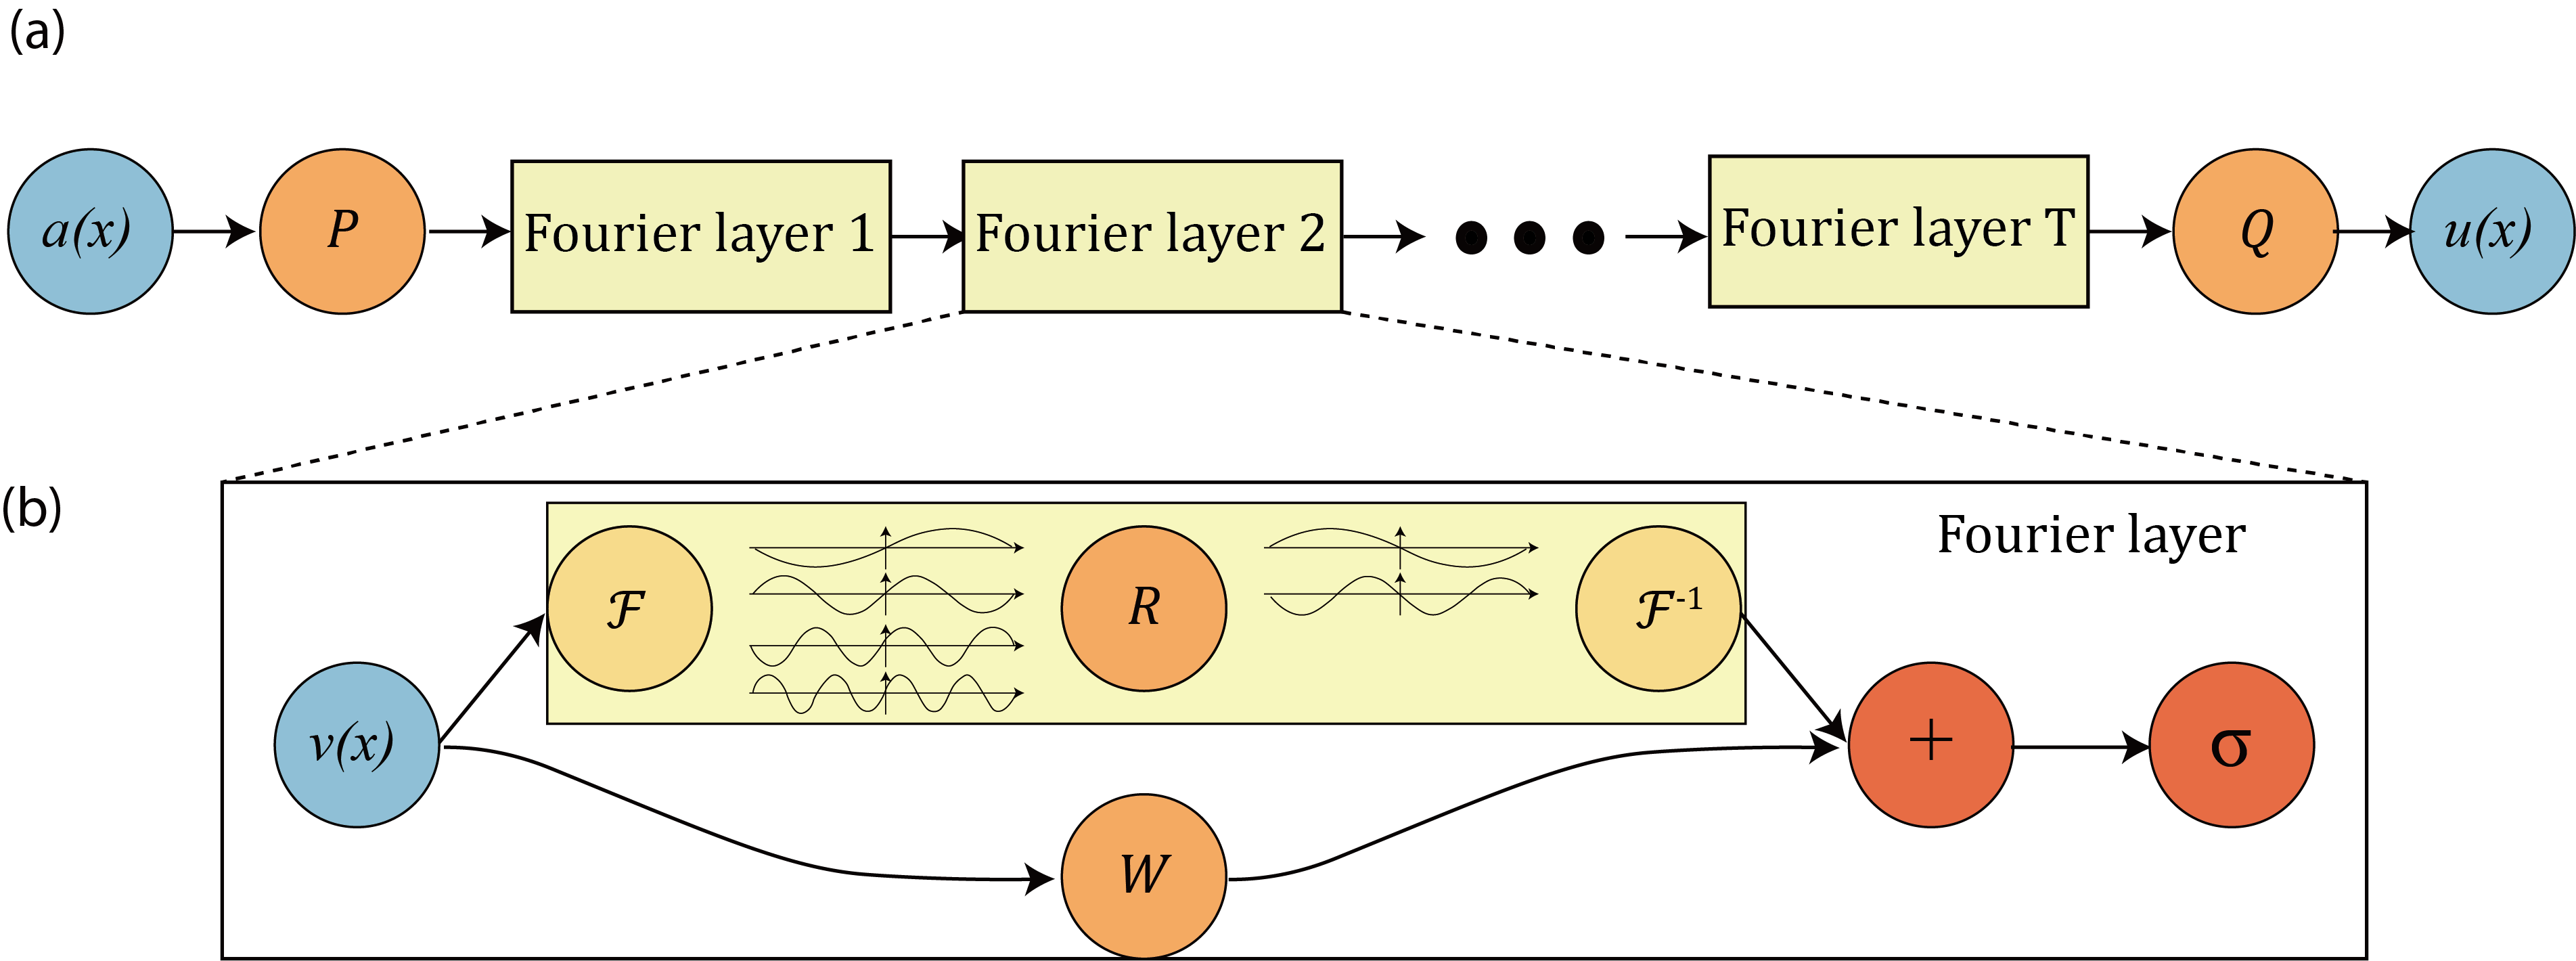
\includegraphics[width=\textwidth]{Figs/fourier_full_arch.png}
        \caption{ {\bf top:} The architecture of the neural operators; \textbf{bottom:} Fourier layer.}
    \label{fig:arch}
    \small{
    {\bf (a) The full architecture of neural operator}: start from input $a$. 1. Lift to a higher dimension channel space by a neural network $\mathcal{P}$. 2. Apply $T$ (typically $T=4$) layers of integral operators and activation functions. 3. Project back to the target dimension by a neural network $Q$. Output $u$.
    {\bf (b) Fourier layers}: Start from input $v$. On top: apply the Fourier transform $\cG$; a linear transform $R$ on the lower Fourier modes which also filters out the higher modes; then apply the inverse Fourier transform $\cG^{-1}$. On the bottom: apply a local linear transform $W$.
    }
\end{figure}

For frequency mode \(k \in \Z^d\), we have $(\cG v)(k) \in \C^{n}$ and $R_\phi(k) \in \C^{m \times n}$. We pick a finite-dimensional parameterization by truncating the Fourier series at a maximal number of modes 
\(k_{\text{max}} = |Z_{k_{\text{max}}}| = |\{k \in \mathbb{Z}^d : |k_j| \leq k_{\text{max},j}, \text{ for } j=1,\dots,d\}|.\) This choice improves the empirical performance and sensitivity of the resulting model with respect to the choices of discretization.
We thus parameterize $R_\phi$ directly as complex-valued $(k_{\text{max}} \times m \times n)$-tensor comprising a collection of truncated Fourier modes and therefore drop $\phi$ from our notation. 
In the case where we have real-valued  \(v\) and we want \(u\) to also be real-valued, we impose that $\kappa$ is real-valued by enforcing conjugate symmetry in the parameterization i.e.
\[R(-k)_{j,l} = R^*(k)_{j,l} \qquad \forall k \in Z_{k_{\text{max}}}, \quad j=1,\dots,m, \:\: l=1,\dots,n.\]
We note that the set $Z_{k_{\text{max}}}$ is not the canonical choice for the low frequency modes of $v_t$. Indeed, the low frequency modes are usually defined by placing an upper-bound on the $\ell_1$-norm of $k \in \mathbb{Z}^d$. We choose $Z_{k_{\text{max}}}$ as above since it allows for an efficient implementation.  Figure~\ref{fig:arch} gives a pictorial representation of an entire Neural Operator architecture employing Fourier layers.

%where the multiplication $\cdot$ is pointwise with respect to the mode $k$.  $(\cG v)(k) \in \C^{d_v}$ is the Fourier transform of $v$ on the mode $k$. $R(k) \in \C^{d_v \times d_v}$ is the weight matrix that is constrained so that the left hand-side of the identity in \eqref{eq:Fourier} is real-valued. We only pass in lower modes $k \leq k_{max}$; higher modes are filter out.
%In words, the Fourier integral operator consists of three steps 1. apply Fourier transformation  $v\mapsto \cG v$. 2. For each mode $k$ smaller than $k_{max}$, multiply $(\cG v)(k)$ with the weight $R(k)$.  Higher modes $(k > k_{max})$ are set to zeros. 3. in the end, apply the inverse Fourier transfer $\cG^{-1}$.
%The flow diagram is shown in Figure \ref{fig:1}.



\paragraph{The Discrete Case and the FFT.}
Assuming the domain $D$ is discretized with $J \in \mathbb{N}$ points, we can treat $v \in \C^{J \times n}$ and $\cG (v) \in \C^{J \times n}$.
Since we convolve $v$ with a function which only has $k_{\text{max}}$ Fourier modes, we may simply truncate the higher modes to obtain $\cG (v) \in \C^{k_{\text{max}} \times n}$. Multiplication by the weight tensor $R \in \C^{k_{\text{max}} \times m \times n}$ is then
%In the discretized case, if the discretization $D_j$ consists of $n$ points, then $v \in \R^{n \times d_v}$,  $k \in \{0,\ldots, n-1\}$, and $\cG v \in \C^{n \times d_v}$.  
%We truncate the modes up to $k_{max}$, so we can also write $\cG v \in \C^{k_{max} \times d_v}$.
%The weight matrix $R \in \C^{k_{max} \times d_v \times d_v}$ is a transformation on the channel dimension $d_v$, separately on each mode $k$:
\begin{equation}
\label{eq:fft_mult}
\bigl( R \cdot (\cG v_t) \bigr)_{k,l} = \sum_{j=1}^{n} R_{k,l,j}  (\cG v)_{k,j}, \qquad k=1,\dots,k_{\text{max}}, \quad l=1,\dots,m.
\end{equation}
%The transformed representation $R \cdot (\cG v)$ will have the same shape as the original one $\cG v \in \C^{n \times d_v}$.\\
When the discretization is uniform with resolution \(s_1 \times  \cdots \times s_d = J\), $\cG$ can be replaced by the Fast Fourier Transform. For $v \in \C^{J \times n}$,   $k = (k_1, \ldots, k_{d}) \in \bbZ_{s_1} \times \cdots \times \bbZ_{s_d}$, and $x=(x_1, \ldots, x_{d}) \in D$, the FFT $\hat{\cG}$ and its inverse $\hat{\cG}^{-1}$ are defined as
\begin{align*}
    (\hat{\cG} v)_l(k) = \sum_{x_1=0}^{s_1-1} \cdots \sum_{x_{d}=0}^{s_d-1} v_l(x_1, \ldots, x_{d}) e^{- 2i \pi \sum_{j=1}^{d} \frac{x_j k_j}{s_j} }, \\
    (\hat{\cG}^{-1} v)_l(x) = \sum_{k_1=0}^{s_1-1} \cdots \sum_{k_{d}=0}^{s_d-1} v_l(k_1, \ldots, k_{d}) e^{2i \pi \sum_{j=1}^{d} \frac{x_j k_j}{s_j} }
\end{align*}
for $l=1,\dots,n$. 
% where we abuse notation and index the rows of the matrix $f$ by either the Fourier mode $k$ or the spatial location $x$ and index the column by the subscript $l$.
In this case, the set of truncated modes becomes
\[Z_{k_{\text{max}}} = \{(k_1, \ldots, k_{d}) \in \bbZ_{s_1} \times \cdots \times \bbZ_{s_d} \mid k_j \leq k_{\text{max},j} \text{ or }\ s_j-k_j \leq k_{\text{max},j}, \text{ for } j=1,\dots,d\}.\]
When implemented, $R$ is treated as a $(s_1 \times \cdots \times s_d \times m \times n)$-tensor and the above definition of $Z_{k_{\text{max}}}$ corresponds to the ``corners'' of $R$, which allows for a straight-forward parallel implementation of (\ref{eq:fft_mult}) via matrix-vector multiplication. 
In practice, we have found the choice $k_{\text{max},j}$ roughly around $\frac{1}{3}$ to $\frac{2}{3}$ of the maximum number of Fourier modes in the Fast Fourier Transform of the grid valuation of the input function provides desirable performance. In our empirical studies, we set $k_{\text{max},j}=12$  which yields $k_{\text{max}} = 12^d$ parameters per channel, to be sufficient for all the tasks that we consider.

%We note, however, that this is not the canonical choice for the low modes which are usually defined by
%\{\}


%lower modes are defined as $\{k = [k_1, \ldots, k_{d}] \mid k_i \leq k_{max,i}\ {\text or}\ s-k_i \leq k_{max,i}, \ {\text for} \ i=1,\ldots,d\}$, which are the ``corners'' of the $s \times \cdots \times s$ matrix (tensor) $Fv$, allowing easy parallel implementation via matrix-vector multiplication. In this case $k_{max} = 2^d \prod k_{max,i}$. Notice we don't use the canonical choice of lower mode ($\sum_i k_i \leq k_{max}$) for implementation reason. In practice, $k_{max,i} = 20,  (k_{max} = 20^d)$ is usually sufficient, no matter the given resolution $s$.


% \paragraph{Truncation of the modes}
% Usually, we don't need all the frequency; the first several modes are sufficient. For a given maximum wave number $k_{max}$, we use only these modes such that $\|k\|_{\infty} \leq k_{max}$, i.e. $k_i < k_{max}$ or $n-k_i < k_{max}$ for all $i$. 
% In other words,   $ R\bigl(k,(\cG a)(k);\phi\bigr)$ is non-zero only if $\|k\|_{\infty} \leq k_{max}$. In practice, $k_{max} = 20$ is sufficient.

% \paragraph{Transform $\cG$.}
% The canonical example of $\cG$ we used in the paper  is the Fourier transform on the unit torus. Other choices of $\cG$ is also possible.
% \begin{align*}
%     (\cG f)(\xi) = \int_{D} f(x) e^{- 2i \pi \langle x, \xi \rangle} \mathrm{d}x \\
%     (\cG^{-1} g)(x) = \int_{D} g(k) e^{2i \pi \langle x, \xi \rangle} \mathrm{d}\xi
% \end{align*}

% For the discretized case, when the discretization is uniform, $\cG$ is replaced by a discrete Fourier transformation. Let $f \in \R^{n,d_v}$, $k = [k_1, \ldots, k_{d_v}] \in \{0,\ldots, n-1\}^{d_v}$
% \begin{align*}
%     (\cG f)[k_1, \ldots, k_{d_v}] = \sum_{j_1=0}^{n-1} \cdots \sum_{j_{d_v}=0}^{n-1} f[j_1, \ldots, j_{d_v}] e^{- 2i \pi \sum_{i=1}^{d_v} \frac{j_i k_i}{n} } \\
%     (\cG g)[j_1, \ldots, j_{d_v}] = \sum_{k_1=0}^{n-1} \cdots \sum_{k_{d_v}=0}^{n-1} g[k_1, \ldots, k_{d_v}] e^{2i \pi \sum_{i=1}^{d_v} \frac{j_i k_i}{n} }
% \end{align*}


\paragraph{Choices for $R$.} In general, $R$ can be defined to depend on $(\cG a)$, the Fourier transform of the input \(a \in \A\) to parallel our construction \eqref{eq:kernelop2}.
Indeed, we can define $R_\phi: \mathbb{Z}^d \times \C^{d_a} \to \C^{m \times n}$
as a parametric function that maps \(\bigl(k,(\cG a)(k))\) to the values of the appropriate Fourier modes. We have experimented with the following parameterizations of $R_\phi$:
\begin{itemize}
    \item \textit{Direct. } Define the parameters $\phi_k \in \C^{m \times n }$ for each wave number $k$:
    \[ R_\phi \bigl(k,(\cG a)(k)\bigr) := \phi_k.\]
    \item \textit{Linear. } Define the parameters \(\phi_{k_1} \in \C^{m \times n \times d_a}\), \(\phi_{k_2} \in \C^{m \times n}\) for each wave number $k$:
    \[R_\phi \bigl(k,(\cG a)(k)\bigr) := \phi_{k_1} (\cG a)(k) + \phi_{k_2}.\]
    \item \textit{Feed-forward neural network.}
    Let $\Phi_\phi:  \mathbb{Z}^d \times \C^{d_a} \to \C^{m \times n}$ be a neural network with parameters $\phi$:
    \[R_\phi \bigl(k,(\cG a)(k)\bigr) := \Phi_\phi(k, (\cG a)(k)). \]
\end{itemize}
We find that the \textit{linear} parameterization has a similar performance to the \textit{direct} parameterization above, \done{use label to point to this direct parameterization}
however, it is not as efficient both in terms of computational complexity and the number of parameters required.
On the other hand, we find that the \textit{feed-forward neural network} parameterization has a worse performance.  This is likely due to the discrete structure of the space $\mathbb{Z}^d;$ numerical evidence suggests neural networks are not adept at handling this structure. Our experiments in this work focus on the direct parameterization presented above.

\iffalse
\paragraph{Activation functions on the spatial domain.} We choose to apply the activation functions on the spatial domain. One can instead directly apply activation functions on the Fourier domain. But in practice, it doesn't work as well, because the pointwise activation function in the Fourier domain is equivalent to spatial convolution, which loses the meaning of the activation functions. We need the activation functions on the spatial domain to recover the higher Fourier modes and non-periodic boundary condition.


\paragraph{Periodic boundary condition.} Traditional Fourier methods work only with periodic boundary conditions, however, our Fourier neural operator does not have this limitation (Darcy and the time domain of Navier-Stokes), because the bias term $W$ in the iterative update helps to keep track of the non-periodic components.

\paragraph{Weight initialization.} The weight initialization is critial for neural network methods (cite). Usually, the weight is initialized from the uniform distribution Uniform$(-1/\sqrt{w}, 1/\sqrt{w})$, where $w$ is the size of the weights in the linear transformation. With the same spirit, we initialize the weight matrix $\bigl( R(\cG a) (\cG v) \bigr)$ of the shape $(d_v, d_v, k_{max})$ by Uniform$(-1/d_v, 1/d_v)$, so that the linear transform roughly preserves the norm of the representation. Notice the wavenumber $k_{max}$ isn't taken into account. Because the transform is done on each wavenumber separately.
\fi

\paragraph{Invariance to Discretization.}
The Fourier layers are discretization-invariant because they can learn from and evaluate functions which are discretized in an arbitrary way. Since parameters are learned directly in Fourier space, resolving the functions in physical space simply amounts to projecting on the basis elements $e^{2\pi i \langle x, k \rangle}$; these are well-defined everywhere on $\C^d$. 
%This allows us to achieve zero-shot super-resolution as shown in Section \ref{sec:superresolution}.
% \nik{Therefore we achieve super-resolution (I'm not sure about this, how it should be stated and if we have an example?)}
% Zongyi: I guess we can leave the example to the experiment section
%Furthermore, our architecture has a consistent error at any resolution of the inputs and outputs. On the other hand, notice that, in Figure \ref{fig:error}, the standard CNN methods we compare against have an error which grows with the resolution.  

%in a sense that it can learn and evaluate on arbitrary resolutions, because the modes $k_{max}$ is fixed and the corresponding basis function $e^{2i\pi \langle x,k\rangle}$ are resolution-invariant.
%When using the general Fourier transform, the Fourier neural operator is also discretization-invariant, while aliasing problem may raise. 
%When the input is uniform and FFT is used, the method will be restricted to uniform grids, but still resolution-invariant if one resolution is a multiple of another.

\paragraph{Quasi-linear Complexity.}
The weight tensor $R$ contains $k_{\text{max}} < J$ modes, so the inner multiplication has complexity $\mathcal{O}(k_{\text{max}})$. Therefore, the majority of the computational cost lies in computing the Fourier transform $\cG(v)$ and its inverse. General Fourier transforms have complexity $\mathcal{O}(J^2)$, however, since we truncate the series the complexity is in fact $\mathcal{O}(J k_{\text{max}})$, while the FFT has complexity $\mathcal{O}(J \log J)$. Generally, we have found using FFTs to be very efficient, however, a uniform discretization is required. 


\paragraph{Non-uniform and Non-periodic Geometry.}
The Fourier neural operator model is defined based on Fourier transform operations accompanied by local residual operations and potentially additive bias function terms. These operations are mainly defined on general geometries, function spaces, and choices of discretization. They are not limited to rectangular domains, periodic functions, or uniform grids. In this paper, we instantiate these operations on uniform grids and periodic functions in order to develop fast implementations that enjoy spectral convergence and utilize methods such as fast Fourier transform. In order to maintain a fast and memory-efficient method, our implementation of the Fourier neural operator relies on the fast Fourier transform which is only defined on uniform mesh discretizations of \(D = \mathbb{T}^d\), or for functions on the square satisfying homogeneous Dirichlet (fast Fourier sine transform) or
homogeneous Neumann (fast Fourier cosine transform) boundary conditions.
However, the fast implementation of Fourier neural operator  can be applied in more general geometries via Fourier continuations. Given any compact manifold $D = \mathcal{M}$, we can always embed it into a periodic cube (torus), 
\[i: \mathcal{M} \to \mathbb{T}^d\]
where the regular FFT can be applied. Conventionally, in numerical analysis
applications, the embedding $i$ is defined through a continuous extension by fitting polynomials \citep{bruno2007accurate}. However, in the Fourier neural operator, the idea can be applied simply by padding the input with zeros. The loss is computed only on the original space during training. The Fourier neural operator will automatically generate a smooth extension to the padded domain in the output space.
